%% TCDimerTreeTopology
%% FigTCDimerTreeTopologyParams.tex
%% Unused packages and definitions removed; TikZ/PGFPlots source formatted.

\documentclass[tikz,margin=2mm]{standalone}
\usetikzlibrary{arrows}

\def\b{\mathsf{b}}
\def\c{\mathsf{c}}
\def\d{\mathsf{d}}

\def\kappab{\kappa_{\b}}
\def\kappac{\kappa_{\c}}
\def\kappad{\kappa_{\d}}

\def\etabb{\eta_{\b\b}}
\def\etabc{\eta_{\b\c}}
\def\etacc{\eta_{\c\c}}
\def\etabd{\eta_{\b\d}}
\def\etacd{\eta_{\c\d}}
\def\etadd{\eta_{\d\d}}

\begin{document}

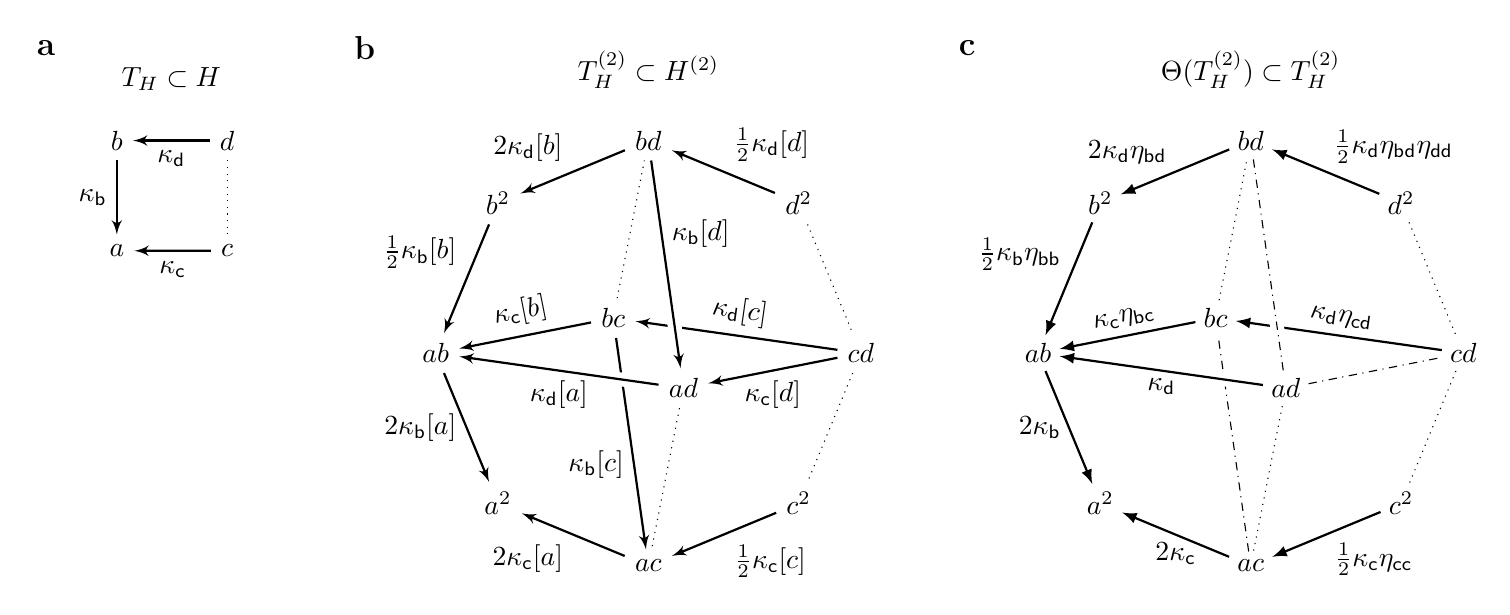
\begin{tikzpicture}[scale=0.9,style=thick,shorten >=0pt,shorten <=0pt,>=latex']

    %\begin{scope}[node distance=1.4cm,xshift=-6cm,yshift=2.7cm]
        %\node (B) {$a_2$};
        %\node[below of = B] (A) {$a_1$};
        %\draw [->,thick] (B) to node[left,align=center] {$e_2$} (A);
        %\node[right of = A] (C) {$a_3$};
        %\draw [<-,thick] (A) to node[below] {$e_3$} (C);
        %\node[right of = B] (D) {$a_4$};
        %\draw [->,thick] (D) to node[below] {$e_4$} (B);
        %\path (B) to node[above,yshift=0.5cm] {$T \subset H $:} (D);
        %\draw [dotted,thin] (C) to (D);
        %\end{scope}

    \begin{scope}[node distance=1.4cm,xshift=-7cm,yshift=3cm]
        \node (B) {$b$};
        \node[below of=B] (A) {$a$};
        \draw[->,thick] (B) to node[left,align=center] {$\kappab$} (A);
        \node[right of=A] (C) {$c$};
        \draw[<-,thick] (A) to node[below] {$\kappac$} (C);
        \node[right of=B] (D) {$d$};
        \draw[->,thick] (D) to node[below] {$\kappad$} (B);
        \draw[dotted,thin] (C) to (D);
        \path (B) to node[above,yshift=0.5cm] {$T_H \subset H $} (D);
    \end{scope}

    \begin{scope}[xshift=0.5cm,yshift=0cm,scale=1,shorten >=0pt,shorten <=0pt]
        \coordinate (title) at (90:4);
        \draw (title) node {$T_H^{(2)} \subset H^{(2)}$};
        \draw (0:3) node[] (cd) {$cd$};
        \draw (45:3) node[] (d2) {$d^2$};
        \draw (90:3) node[] (bd) {$bd$};
        \draw (135:3) node[] (b2) {$b^2$};
        \draw (180:3) node[] (ab) {$ab$};
        \draw (225:3) node[] (a2) {$a^2$};
        \draw (270:3) node[] (ac) {$ac$};
        \draw (315:3) node[] (c2) {$c^2$};
        \draw (315:0.7) node[] (ad) {$ad$};
        \draw (135:0.7) node[] (bc) {$bc$};
        \draw[<-,thick] (a2) -- node[left] {$2\kappab[a]$} (ab);
        \draw[<-,thick] (ab) -- node[above left] {$\frac{1}{2}\kappab[b]$} (b2);
        \draw[<-,thick] (b2) --  node[pos=0.75] (b2bd) {} node[above left] {$2\kappad[b]$} (bd);
        \draw[<-,thick] (bd) -- node[above right] {$\frac{1}{2}\kappad[d] $} (d2);
        \draw[thin,dotted] (d2) -- (cd);
        \draw[thin,dotted] (cd) -- (c2);
        \draw[<-,thick] (ac) -- node[below right] {$\frac{1}{2}\kappac [c]$} (c2);
        \draw[->,thick] (ac) -- node[below left] {$2\kappac[a]$} (a2);
        \draw[thin,dotted] (bc) -- (bd);
        \draw[thin,dotted] (ad) -- (ac);
        \draw[<-,thick] (ab) --  node[above,sloped] {$\kappac[b]$} (bc);
        \draw[<-,thick] (bc) -- node[above,sloped] {$\kappad[c] $} (cd);
        %\draw[thin,dashdotted] (ad) --  (cd);
        %\draw[<-,thin,dashdotted] (ad) -- node[below,pos=0.5]  {$\kappac[d]$}  (cd);
        \draw[<-,thick] (ad) -- node[below,pos=0.5]  {$\kappac[d]$}  (cd);
        %\draw[thin,dashdotted] (ad) -- node[pos=0.75] (adbd) {} (bd);
        \draw[white,line width=5pt] (ad) -- node[pos=0.75] (adbd) {} (bd);
        %\draw[<-,thin,dashdotted] (ad) -- node[pos=0.65,right] (adbd) {$\kappab[d]$} (bd);
        \draw[<-,thick] (ad) -- node[pos=0.65,right] (adbd) {$\kappab[d]$} (bd);
        %\draw[thin,dashdotted] (ac) -- node[pos=0.75] (bcac) {} (bc);
        %\draw[<-, thin,dashdotted] (ac) -- node[left,pos=0.4] (bcac) {$\kappab[c]$} (bc);
        \draw[<-, thick] (ac) -- node[left,pos=0.4] (bcac) {$\kappab[c]$} (bc);
        \draw[white,line width=5pt] (ab) -- node[below] {$\kappad[a]$} (ad);
        \draw[<-,thick] (ab) -- node[below] {$\kappad[a]$} (ad);
    \end{scope}

    \begin{scope}[xshift=9cm,yshift=0cm,scale=1,shorten >=0pt,shorten <=0pt,outer sep=1pt,inner sep=2pt,>=latex]
        \coordinate (title) at (90:4);
        \draw (title) node {$\Theta(T_H^{(2)}) \subset T_H^{(2)}$};
        \draw (0:3) node[] (cd) {$cd$};
        \draw (45:3) node[] (d2) {$d^2$};
        \draw (90:3) node[] (bd) {$bd$};
        \draw (135:3) node[] (b2) {$b^2$};
        \draw (180:3) node[] (ab) {$ab$};
        \draw (225:3) node[] (a2) {$a^2$};
        \draw (270:3) node[] (ac) {$ac$};
        \draw (315:3) node[] (c2) {$c^2$};
        \draw (315:0.7) node[] (ad) {$ad$};
        \draw (135:0.7) node[] (bc) {$bc$};
        \draw[<-,thick] (a2) -- node[left] {$2\kappab$} (ab);
        \draw[<-,thick] (ab) -- node[above left] {$\frac{1}{2}\kappab\etabb$} (b2);
        \draw[<-,thick] (b2) --  node[pos=0.75] (b2bd) {} node[above left] {$2\kappad\etabd$} (bd);
        \draw[<-,thick] (bd) -- node[above right] {$\frac{1}{2}\kappad \etabd\etadd$} (d2);
        \draw[thin,dotted] (d2) -- (cd);
        \draw[thin,dotted] (cd) -- (c2);
        \draw[<-,thick] (ac) -- node[below right] {$\frac{1}{2}\kappac \etacc $} (c2);
        \draw[->,thick] (ac) -- node[below] {$2\kappac$} (a2);
        \draw[thin,dotted] (bc) -- (bd);

        \draw[thin,dotted] (ad) -- (ac);
        \draw[thin,dashdotted] (ac) -- node[pos=0.75] (bcac) {} (bc);
        \draw[<-,thick] (ab) --  node[above,sloped] {$\kappac \etabc$} (bc);
        \draw[<-,thick] (bc) -- node[above,sloped] {$\kappad \etacd$} (cd);
        \draw[thin,dashdotted] (ad) --  (cd);

        \draw[white,line width=5pt] (ab) -- node[below] {} (ad);
        \draw[<-,thick] (ab) -- node[below] {$\kappad$} (ad);

        \draw[white,line width=5pt] (ad) -- node[pos=0.75] (adbd) {} (bd);
        \draw[thin,dashdotted] (ad) -- node[pos=0.75] (adbd) {} (bd);
    \end{scope}

    \def\height{4.3}
    \def\left{-8}
    \draw (\left,\height) node[font=\large] {{\bf a}};
    \draw (\left+4.5,\height) node[font=\large] {{\bf b}};
    \draw (\left+13,\height) node[font=\large] {{\bf c}};

\end{tikzpicture}

\end{document}

